% !TeX root = ../main.tex
\subsection{问题四：次品率带抽样不确定性的重决策}

\subsubsection{任务与建模思路}

问题四把问题二表~1 与问题三表~2 中的全部次品率视为通过抽样检测方法得到的估计值，要求在此基础上重新完成问题二与问题三的决策。与前三问相比，本问不再把标称次品率当作已知常数，而是显式保留“抽样只提供有限证据”这一不确定性：给定同样的样本结果，真实次品率仍可能明显偏离样本比例，策略必须同时权衡所有可能的真实参数。

本文的处理分两层。第一层把每个次品率转化为后验分布：将表~1、表~2 中的数值解释为 $n$ 件样本中检出的次品比例，在无信息均匀先验下得到 Beta 后验。第二层用后验情景平均计算每个策略的期望利润：从各环节后验分布抽取 $S$ 组联合参数情景，在每个情景下按 5.2 节与 5.3 节相同的质量传递与成本规则解析计算利润，再对情景取平均。决策准则为风险中性的后验期望利润最大化，标准差与 $5\%$ 分位数作为风险描述指标辅助刻画方案的收益波动与下行风险，不进入目标函数。

题面未给出实际抽样样本量 $n$。本文将 $n$ 作为证据强度参数：数值示例选取能够兼容题面各名义次品率（$k=np$ 为整数）的 $n=40$ 作为代表性小样本情景，并进一步考察 $n=100,200,1000,10000$ 的变化，以说明抽样证据量对决策的影响。该设定在 3 节假设表中单独列出，企业提供真实抽样方案后可直接替换重算。

问题二的重决策在 5.2.5 节定义的七变量固定策略类 $\{0,1\}^7$ 中进行，与点估计口径的固定决策基准属于同一策略类；问题三在 $\{0,1\}^{16}$ 中完全枚举，遗传算法仅作策略空间扩大后的扩展验证。

\subsubsection{Beta 后验与情景平均}

设某环节的名义次品率为 $\hat p$，并假设该值来自 $n$ 件样本中的 $k=n\hat p$ 件次品。观测模型为 $k\sim\operatorname{Bin}(n,p)$，在无信息先验 $p\sim\operatorname{Beta}(1,1)$ 下，后验为
\begin{equation}
  \pi(p\mid k,n)=\operatorname{Beta}(k+1,n-k+1),
  \label{eq:q4-posterior}
\end{equation}
后验均值为
\begin{equation}
  \mathbb{E}[p\mid k,n]=\frac{k+1}{n+2}.
  \label{eq:q4-posterior-mean}
\end{equation}
在本题名义值均小于 $0.5$ 的范围内，式~\eqref{eq:q4-posterior-mean} 严格大于样本比例 $\hat p=k/n$。因此后验期望利润低于点估计口径的下降来自两个可分离的效应：一是均匀先验与有限样本共同造成的后验均值向 $0.5$ 收缩（均值偏移），二是后验本身围绕均值存在的参数波动（不确定性）；前者使基准利润水平系统性下移，后者使利润出现情景间波动，两者不能混为一谈。以 $n=40$ 为例，$5\%$、$10\%$、$20\%$ 三个名义值分别对应 $\operatorname{Beta}(3,39)$、$\operatorname{Beta}(5,37)$、$\operatorname{Beta}(9,33)$，其均值、标准差与 $95\%$ 后验区间见表~\ref{tab:q4-posterior}，图~\ref{fig:q4-posterior-convergence}(a) 给出三条后验密度曲线。Beta 后验及其矩性质属于贝叶斯统计的标准结果\cite{bayes-gelman,stat-casella}。

\begin{table}[H]
  \centering
  \caption{$n=40$ 时名义次品率对应的 Beta 后验统计量}
  \label{tab:q4-posterior}
  \begin{tabular}{cccccc}
    \toprule
    名义次品率 $\hat p$ & 样本次品数 $k$ & 后验分布 & 后验均值 & 后验标准差 & $95\%$ 后验区间 \\
    \midrule
    $0.05$ & $2$ & $\operatorname{Beta}(3,39)$ & $0.0714$ & $0.0393$ & $[0.0154,0.1653]$ \\
    $0.10$ & $4$ & $\operatorname{Beta}(5,37)$ & $0.1190$ & $0.0494$ & $[0.0408,0.2313]$ \\
    $0.20$ & $8$ & $\operatorname{Beta}(9,33)$ & $0.2143$ & $0.0626$ & $[0.1056,0.3487]$ \\
    \bottomrule
  \end{tabular}
\end{table}

设 $\theta$ 汇集某一情形下全部不确定的次品率，$\Pi(X,\theta)$ 为策略 $X$ 在参数 $\theta$ 下的解析期望利润。从后验中抽取 $S=10000$ 组情景 $\theta^{(s)}$，定义后验期望利润
\begin{equation}
  \bar\Pi(X)=\frac{1}{S}\sum_{s=1}^{S}\Pi(X,\theta^{(s)}),
  \label{eq:q4-expected-profit}
\end{equation}
利润标准差
\begin{equation}
  \sigma(X)=\sqrt{\frac{1}{S}\sum_{s=1}^{S}\bigl[\Pi(X,\theta^{(s)})-\bar\Pi(X)\bigr]^2},
  \label{eq:q4-profit-sd}
\end{equation}
并以情景利润的 $5\%$ 经验分位数 $q_{0.05}(X)$ 刻画下行风险。重决策目标为
\begin{equation}
  X^\ast=\arg\max_{X}\bar\Pi(X),
  \label{eq:q4-objective}
\end{equation}
其中问题二枚举七变量固定策略类的全部 $2^7=128$ 个策略，问题三完全枚举 $\{0,1\}^{16}$。所有策略在同一组后验情景上评估，比较口径一致；内层生产期望沿用解析递推而非二次模拟，避免在参数情景之上叠加蒙特卡洛误差。

随着样本量增大，后验 $\operatorname{Beta}(k+1,n-k+1)$ 围绕名义值收缩，式~\eqref{eq:q4-expected-profit} 应收敛到点估计口径 $\Pi(X;p_0)$。该性质同时用作程序正确性与模型一致性的检验：若小样本下策略发生切换而大样本下恢复，说明切换由参数不确定性引起，而非数值噪声。

\subsubsection{问题二重决策：后验情景下的七变量固定策略}

问题二在七变量固定策略类中重决策，七个决策位依次为零配件 1、零配件 2 首次是否检测、首次是否检测成品、不合格成品是否拆解、拆解回收后零配件 1、零配件 2 是否检测，以及拆解后再装配是否检测成品；该策略类与 5.2.5 节的七变量固定基准完全一致。表~\ref{tab:q4-q2} 给出 $n=40$ 时六种情形的点估计最优策略与后验最优策略。

\begin{table}[H]
  \centering
  \caption{$n=40$ 时问题二七变量固定策略的点估计与后验最优结果}
  \label{tab:q4-q2}
  \small
  \begin{tabular}{c>{\raggedright\arraybackslash}p{0.15\textwidth}>{\raggedright\arraybackslash}p{0.15\textwidth}rrrc}
    \toprule
    情形 & 点估计最优策略 & 后验最优策略 & 后验利润/元 & 标准差/元 & $5\%$ 分位/元 & 切换 \\
    \midrule
    1 & $1001010$ & $1001010$ & $18.3806$ & $1.2983$ & $15.9833$ & 否 \\
    2 & $1101000$ & $1101000$ & $11.4397$ & $1.8554$ & $8.0765$ & 否 \\
    3 & $1011011$ & $1011011$ & $16.1395$ & $1.0918$ & $14.0787$ & 否 \\
    4 & $1111001$ & $1111001$ & $14.3518$ & $1.3766$ & $11.8008$ & 否 \\
    5 & $0101100$ & $0111100$ & $14.7880$ & $1.3607$ & $12.2706$ & 是 \\
    6 & $0000000$ & $0000000$ & $20.5654$ & $1.9965$ & $16.7734$ & 否 \\
    \bottomrule
  \end{tabular}
\end{table}

六种情形的后验期望利润均低于点估计口径，例如情形 1 由 $18.9222$ 元降至 $18.3806$ 元，情形 6 由 $21.6787$ 元降至 $20.5654$ 元，来源是后验均值相对名义值的上移与参数波动的共同作用。策略切换集中在情形 5：点估计最优策略 $0101100$（检零配件 2、拆解但不检成品）在参数不确定性下变为 $0111100$，即补上成品检测；其余情形在七变量策略类内保持原方案。与仅含四个变量的受限类相比，七变量类允许拆解后再检测与再装配检测，多数情形无需改变决策即可吸收参数不确定性，因此切换更少，也说明问题二与问题四的决策类继承是一致的。

风险指标进一步给出决策余地：情形 2 的利润标准差最大（$1.8554$ 元），$5\%$ 分位数为 $8.0765$ 元，表明不利参数情景下利润下降较多；情形 3 标准差最小（$1.0918$ 元），全检测拆解方案的利润波动较低。

\subsubsection{问题三重决策：后验情景下的固定策略最优}

问题三在 $n=40$ 的后验情景下枚举全部 $65536$ 个策略，所得最优策略与点估计口径一致，仍为\allowbreak 1111111111111101\allowbreak；后验期望利润为 $55.0311$ 元，较点估计口径 $60.2222$ 元下降 $5.1912$ 元，利润标准差 $4.8719$ 元，$5\%$ 分位数 $46.3372$ 元。策略含义与问题三相同：全部零配件与半成品检测、不合格半成品拆解、成品不检测、不合格成品拆解；参数不确定性改变的是期望利润水平与风险，而非固定策略空间内的最优结构。

从后验口径的排名看，第二名策略\allowbreak $1111111111111111$\allowbreak（成品也检测）的后验期望利润为 $53.7831$ 元，与最优策略相差 $1.2480$ 元；点估计口径下两者相差 $2.2222$ 元。不确定性使相邻高利润策略的差距被压缩，但最优策略仍可辨识。

\subsubsection{先验与情景数稳定性检验}

为检验策略结论是否依赖均匀先验的选择，在 $n=40$ 下改用 Jeffreys 先验 $\operatorname{Beta}(\tfrac12,\tfrac12)$ 重算：后验变为 $\operatorname{Beta}(k+\tfrac12,n-k+\tfrac12)$，后验均值向名义值收缩更少。结果显示，问题三最优策略仍为 $1111111111111101$（后验期望利润 $57.2994$ 元），问题二情形 1--4、6 的策略均不变；情形 5 在均匀先验下补检成品（$0111100$），在 Jeffreys 先验下保持 $0101100$。因此，除情形 5 外，不同弱信息先验下的最优策略保持一致；情形 5 位于策略切换边界附近，对先验选择敏感，不能将其切换解释为稳健结论。

为检验后验情景数 $S$ 的数值稳定性，在 $n=40$ 下取 $S=1000,5000,10000,20000$ 四档重算。表~\ref{tab:q4-scenario-stability} 显示，问题三最优策略始终为\allowbreak 1111111111111101\allowbreak，后验期望利润随 $S$ 增大稳定在 $55.03$ 元附近，标准差稳定在 $4.87$ 元附近；问题二情形 5 的切换在四个情景数下均出现，其余情形策略不变。$S=10000$ 的结论对情景数不敏感。

\begin{table}[H]
  \centering
  \caption{后验情景数对问题三最优策略与期望利润的影响（$n=40$）}
  \label{tab:q4-scenario-stability}
  \begin{tabular}{crrrr}
    \toprule
    情景数 $S$ & 最优策略 & 期望利润/元 & 标准差/元 & $5\%$ 分位数/元 \\
    \midrule
    $1000$ & $1111111111111101$ & $55.1056$ & $4.6696$ & $47.0323$ \\
    $5000$ & $1111111111111101$ & $55.0573$ & $4.8593$ & $46.3376$ \\
    $10000$ & $1111111111111101$ & $55.0311$ & $4.8719$ & $46.3372$ \\
    $20000$ & $1111111111111101$ & $55.0306$ & $4.8634$ & $46.1718$ \\
    \bottomrule
  \end{tabular}
\end{table}

\subsubsection{样本量收敛与稳定性验证}

为检验抽样证据量对结论的影响，将 $n$ 依次取 $40,100,200,1000,10000$ 重算。图~\ref{fig:q4-posterior-convergence}(b) 与表~\ref{tab:q4-sample-sizes} 显示，问题三的最优策略始终为\allowbreak $1111111111111101$\allowbreak，后验期望利润由 $55.0311$ 元单调上升至 $60.2018$ 元，标准差由 $4.8719$ 元降至 $0.2687$ 元，逐步接近点估计结果 $60.2222$ 元；这与后验分布随 $n$ 收缩的理论性质一致，说明抽样量足够大时本问结论退化为问题三的确定性口径。

\begin{figure}[H]
  \centering
  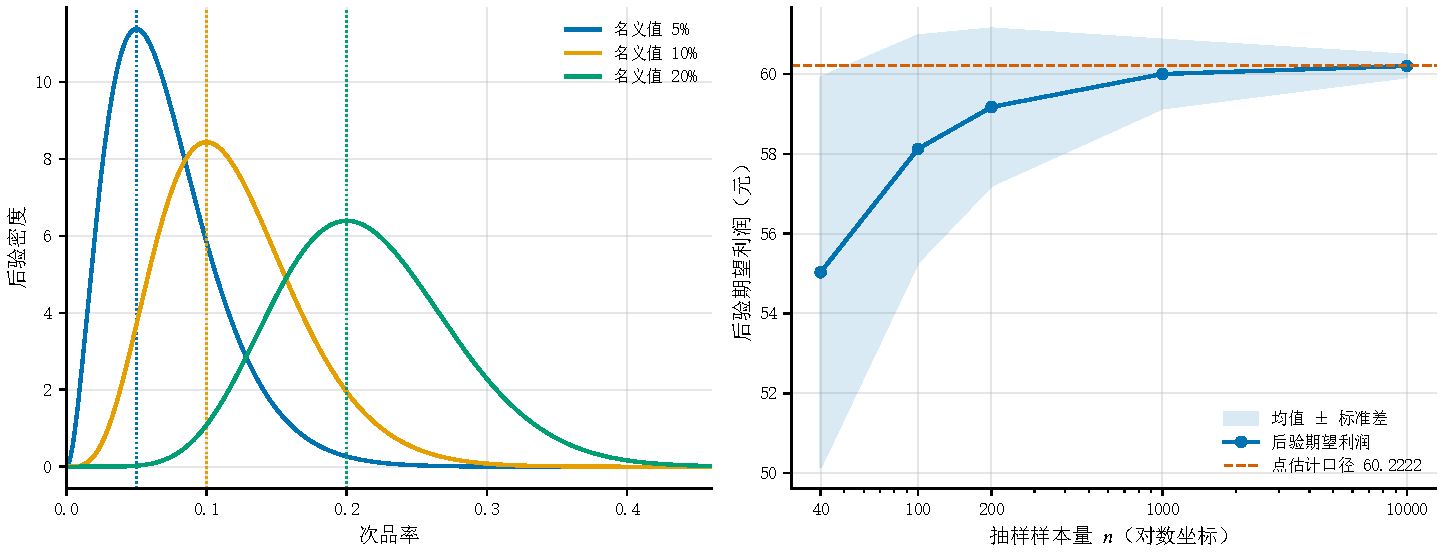
\includegraphics[width=0.98\textwidth]{../../figures/q4/fig_q4_posterior_convergence.pdf}
  \caption{问题四的 Beta 后验分布与样本量收敛}
  \label{fig:q4-posterior-convergence}
\end{figure}

\begin{table}[H]
  \centering
  \caption{问题三最优策略随抽样样本量的收敛}
  \label{tab:q4-sample-sizes}
  \begin{tabular}{crrrr}
    \toprule
    样本量 $n$ & 后验最优策略 & 期望利润/元 & 标准差/元 & $5\%$ 分位数/元 \\
    \midrule
    $40$ & $1111111111111101$ & $55.0311$ & $4.8719$ & $46.3372$ \\
    $100$ & $1111111111111101$ & $58.1226$ & $2.8336$ & $53.2667$ \\
    $200$ & $1111111111111101$ & $59.1740$ & $1.9565$ & $55.8125$ \\
    $1000$ & $1111111111111101$ & $59.9999$ & $0.8504$ & $58.5641$ \\
    $10000$ & $1111111111111101$ & $60.2018$ & $0.2687$ & $59.7555$ \\
    \bottomrule
  \end{tabular}
\end{table}

问题二方面，定义稳定样本量为“从该样本量起，其后所有网格样本量上的后验最优策略均属于点估计最优策略集合”。七变量策略类下六种情形的稳定样本量依次为 $40,40,40,40,80,40$：前四种情形与情形 6 在 $n=40$ 时已与点估计口径一致，情形 5 需要约 $80$ 件样本才恢复点估计最优策略。该结果量化了小样本下参数不确定性实质改变问题二决策的边界：抽样量不足时直接套用点估计策略可能选择次优动作。

\subsubsection{本问小结}

在“表~1、表~2 次品率来自 $n=40$ 件样本的抽样检测”这一代表性小样本情景下，本文以后验期望利润为风险中性准则重做决策：问题二仅情形 5 在七变量策略类内由 $0101100$ 切换为 $0111100$（补检成品），并在 $n=80$ 时恢复点估计策略；问题三最优策略保持 $1111111111111101$，后验期望利润 $55.0311$ 元、标准差 $4.8719$ 元。样本量增大时两类结果均收敛到确定性口径；除情形 5 这一先验敏感的策略边界外，其余策略对弱信息先验与情景数变化保持一致。企业提供实际抽样样本量与跨环节联合抽样数据后，可用真实后验替换 $n=40$ 代表情景。
